\documentclass{beamer}
\usepackage[utf8]{inputenc}

\usetheme{Madrid}
\usecolortheme{default}
\usepackage{amsmath,amssymb,amsfonts,amsthm}
\usepackage{txfonts}
\usepackage{tkz-euclide}
\usepackage{listings}
\usepackage{adjustbox}
\usepackage{array}
\usepackage{tabularx}
\usepackage{gvv}
\usepackage{lmodern}
\usepackage{circuitikz}
\usepackage{tikz}
\usepackage{graphicx}

\setbeamertemplate{page number in head/foot}[totalframenumber]

\usepackage{tcolorbox}
\tcbuselibrary{minted,breakable,xparse,skins}



\definecolor{bg}{gray}{0.95}
\DeclareTCBListing{mintedbox}{O{}m!O{}}{%
  breakable=true,
  listing engine=minted,
  listing only,
  minted language=#2,
  minted style=default,
  minted options={%
    linenos,
    gobble=0,
    breaklines=true,
    breakafter=,,
    fontsize=\small,
    numbersep=8pt,
    #1},
  boxsep=0pt,
  left skip=0pt,
  right skip=0pt,
  left=25pt,
  right=0pt,
  top=3pt,
  bottom=3pt,
  arc=5pt,
  leftrule=0pt,
  rightrule=0pt,
  bottomrule=2pt,
  toprule=2pt,
  colback=bg,
  colframe=orange!70,
  enhanced,
  overlay={%
    \begin{tcbclipinterior}
    \fill[orange!20!white] (frame.south west) rectangle ([xshift=20pt]frame.north west);
    \end{tcbclipinterior}},
  #3,
}
\lstset{
    language=C,
    basicstyle=\ttfamily\small,
    keywordstyle=\color{blue},
    stringstyle=\color{orange},
    commentstyle=\color{green!60!black},
    numbers=left,
    numberstyle=\tiny\color{gray},
    breaklines=true,
    showstringspaces=false,
}
%------------------------------------------------------------
%This block of code defines the information to appear in the
%Title page
\title %optional
{1.4.12}
\date{August 21,2025}
%\subtitle{A short story}

\author % (optional)
{Stalin-AI25BTECH11037}



\begin{document}


\frame{\titlepage}
\begin{frame}{Question}
In what ratio does the point \( P(-4, 6) \) divide the line segment joining the points \( A(-6, 0) \) and \( C(3, -8) \) 
\end{frame}

\begin{frame}{Theoritical Solution}

Given Points
\begin{align*}
\vec{A} = \myvec{-6 \\ 0}, \quad
\vec{C} =  \myvec{3 \\ -8}, \quad
\vec{P} = \myvec{-4 \\ 6},
\end{align*}

the ratio \( k \) in which \( P \) divides \( AC \) is
\[
k = \frac{(\vec{A} - \vec{P})^T (\vec{P} - \vec{C})}{\|\vec{P} - \vec{C}\|^2}
\]

\end{frame}







\begin{frame}{Theoritical Solution}

\begin{align*}
=\frac{ 
 \myvec{-6 + 4 \\ 0 - 6}^T
 \myvec{-4 - 3 \\ 6 + 8}
}{
(-4 - 3)^2 + (6 + 8)^2
}
\end{align*}

\begin{align*}
=\frac{
 \myvec{-2 \\ -6}^T
 \myvec{-7 \\ 14}
}{
(-7)^2 + 14^2
}
\end{align*}
\end{frame}




\begin{frame}{Theoritical Solution}

\textbf{Therefore,}

\begin{align*}
k = \frac{-70}{245} = -\frac{2}{7}
\end{align*}


Since \( k = -\frac{2}{7} \), Point \( P \) divides the segment \( AC \) \textbf{externally} in the ratio \( 2 : 7 \).

\end{frame}


\begin{frame}[fragile]
    \frametitle{C Code - Internal division formula}

    \begin{lstlisting}

#include <stdio.h>
#include <math.h>

int main() {
    // Given points
    double Ax = -6, Ay = 0;
    double Cx = 3,  Cy = -8;
    double Px = -4, Py = 6;

    // Compute vectors (A - P) and (P - C)
    double APx = Ax - Px;
    double APy = Ay - Py;
    double PCx = Px - Cx;
    double PCy = Py - Cy;

    // Dot product (A - P)T(P - C)
    double dot = APx * PCx + APy * PCy;

    \end{lstlisting}
\end{frame}

\begin{frame}[fragile]
    \frametitle{C Code - Internal division formula}

    \begin{lstlisting}

    // Norm squared of (P - C)
    double norm_sq = PCx * PCx + PCy * PCy;

    // Ratio k
    double k = dot / norm_sq;

    printf("The value of k = %.3f\n", k);

    if (k > 0 && fabs(k - floor(k)) < 1e-6) {
        printf("Point P divides AC internally.\n");
    } else if (k < 0) {
        printf("Point P divides AC externally.\n");
    } else {
        printf("Point P does not divide AC.\n");
    }

    return 0;
}


    \end{lstlisting}
\end{frame}

\begin{frame}[fragile]
     \frametitle{Python Code}
     \begin{lstlisting}
         
import math

# Given points
A = (-6, 0)
C = (3, -8)
P = (-4, 6)

# Function to check collinearity using area of triangle
def are_collinear(A, C, P):
    (x1, y1), (x2, y2), (x3, y3) = A, C, P
    # Area of triangle formula: 0 if collinear
    area = x1*(y2-y3) + x2*(y3-y1) + x3*(y1-y2)
    return area == 0

# Function to compute ratio if collinear
def division_ratio(A, C, P):
    (x1, y1), (x2, y2), (x3, y3) = A, C, P
    # Internal/external division formula
    # P divides AC in ratio m:n if (x3,y3) = (m*x2+n*x1)/(m+n), (m*y2+n*y1)/(m+n)
    # We solve for m:n
    if x1 == x2:  # vertical line
        return (y3-y1, y2-y3)
    else:
        return (x3-x1, x2-x3)
        
\end{lstlisting}
\end{frame}


\begin{frame}[fragile]
     \frametitle{Python Code}
     \begin{lstlisting}
     
# Check
if are_collinear(A, C, P):
    m, n = division_ratio(A, C, P)
    if m*n > 0:
        print(f"P divides AC internally in ratio {abs(m)}:{abs(n)}")
    else:
        print(f"P divides AC externally in ratio {abs(m)}:{abs(n)}")
else:
    print("P does not divide AC (points are not collinear





































\end{lstlisting}
\end{frame}



\begin{frame}[fragile]
\frametitle{Python+C Code}
\begin{lstlisting}
    

import math

# Given points
A = (-6, 0)
C = (3, -8)
P = (-4, 6)

# Step 1: Compute vectors
AP = (A[0] - P[0], A[1] - P[1])
PC = (P[0] - C[0], P[1] - C[1])

# Step 2: Dot product and norm squared
dot = AP[0] * PC[0] + AP[1] * PC[1]
norm_sq = PC[0]**2 + PC[1]**2


\end{lstlisting}
\end{frame}

\begin{frame}[fragile]
\frametitle{Python+C Code}
\begin{lstlisting}
    
k = dot / norm_sq

print(f"Computed k = {k:.3f}")

# Step 3: Collinearity check (area of triangle)
area = A[0]*(C[1]-P[1]) + C[0]*(P[1]-A[1]) + P[0]*(A[1]-C[1])

if area == 0:
    if k < 0:
        print(f"P divides AC externally in ratio {abs(int(k*7))}:{7}")
    else:
        print(f"P divides AC internally in ratio {abs(int(k*7))}:{7}")
else:
    print("P is not collinear with A and C, so it does not divide AC.")

\end{lstlisting}
\end{frame}


\begin{frame}{plot}
\begin{figure}[H!]
    \centering
    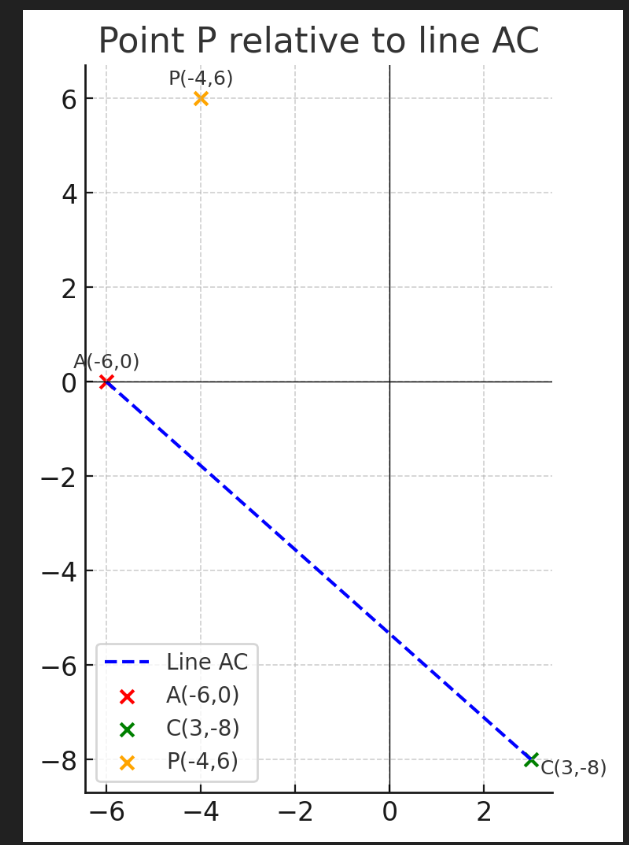
\includegraphics[width=0.5\linewidth]{Fig1.png}
    \caption{Caption}
    \label{fig:placeholder}
\end{figure}

\end{frame}
    





\end{document}